% Options for packages loaded elsewhere
\PassOptionsToPackage{unicode}{hyperref}
\PassOptionsToPackage{hyphens}{url}
%
\documentclass[
]{article}
\usepackage{amsmath,amssymb}
\usepackage{lmodern}
\usepackage{iftex}
\ifPDFTeX
  \usepackage[T1]{fontenc}
  \usepackage[utf8]{inputenc}
  \usepackage{textcomp} % provide euro and other symbols
\else % if luatex or xetex
  \usepackage{unicode-math}
  \defaultfontfeatures{Scale=MatchLowercase}
  \defaultfontfeatures[\rmfamily]{Ligatures=TeX,Scale=1}
\fi
% Use upquote if available, for straight quotes in verbatim environments
\IfFileExists{upquote.sty}{\usepackage{upquote}}{}
\IfFileExists{microtype.sty}{% use microtype if available
  \usepackage[]{microtype}
  \UseMicrotypeSet[protrusion]{basicmath} % disable protrusion for tt fonts
}{}
\makeatletter
\@ifundefined{KOMAClassName}{% if non-KOMA class
  \IfFileExists{parskip.sty}{%
    \usepackage{parskip}
  }{% else
    \setlength{\parindent}{0pt}
    \setlength{\parskip}{6pt plus 2pt minus 1pt}}
}{% if KOMA class
  \KOMAoptions{parskip=half}}
\makeatother
\usepackage{xcolor}
\IfFileExists{xurl.sty}{\usepackage{xurl}}{} % add URL line breaks if available
\IfFileExists{bookmark.sty}{\usepackage{bookmark}}{\usepackage{hyperref}}
\hypersetup{
  pdftitle={Final Term Project 2022-R01},
  pdfauthor={Kwon, Donghoon},
  hidelinks,
  pdfcreator={LaTeX via pandoc}}
\urlstyle{same} % disable monospaced font for URLs
\usepackage[margin=1in]{geometry}
\usepackage{color}
\usepackage{fancyvrb}
\newcommand{\VerbBar}{|}
\newcommand{\VERB}{\Verb[commandchars=\\\{\}]}
\DefineVerbatimEnvironment{Highlighting}{Verbatim}{commandchars=\\\{\}}
% Add ',fontsize=\small' for more characters per line
\usepackage{framed}
\definecolor{shadecolor}{RGB}{248,248,248}
\newenvironment{Shaded}{\begin{snugshade}}{\end{snugshade}}
\newcommand{\AlertTok}[1]{\textcolor[rgb]{0.94,0.16,0.16}{#1}}
\newcommand{\AnnotationTok}[1]{\textcolor[rgb]{0.56,0.35,0.01}{\textbf{\textit{#1}}}}
\newcommand{\AttributeTok}[1]{\textcolor[rgb]{0.77,0.63,0.00}{#1}}
\newcommand{\BaseNTok}[1]{\textcolor[rgb]{0.00,0.00,0.81}{#1}}
\newcommand{\BuiltInTok}[1]{#1}
\newcommand{\CharTok}[1]{\textcolor[rgb]{0.31,0.60,0.02}{#1}}
\newcommand{\CommentTok}[1]{\textcolor[rgb]{0.56,0.35,0.01}{\textit{#1}}}
\newcommand{\CommentVarTok}[1]{\textcolor[rgb]{0.56,0.35,0.01}{\textbf{\textit{#1}}}}
\newcommand{\ConstantTok}[1]{\textcolor[rgb]{0.00,0.00,0.00}{#1}}
\newcommand{\ControlFlowTok}[1]{\textcolor[rgb]{0.13,0.29,0.53}{\textbf{#1}}}
\newcommand{\DataTypeTok}[1]{\textcolor[rgb]{0.13,0.29,0.53}{#1}}
\newcommand{\DecValTok}[1]{\textcolor[rgb]{0.00,0.00,0.81}{#1}}
\newcommand{\DocumentationTok}[1]{\textcolor[rgb]{0.56,0.35,0.01}{\textbf{\textit{#1}}}}
\newcommand{\ErrorTok}[1]{\textcolor[rgb]{0.64,0.00,0.00}{\textbf{#1}}}
\newcommand{\ExtensionTok}[1]{#1}
\newcommand{\FloatTok}[1]{\textcolor[rgb]{0.00,0.00,0.81}{#1}}
\newcommand{\FunctionTok}[1]{\textcolor[rgb]{0.00,0.00,0.00}{#1}}
\newcommand{\ImportTok}[1]{#1}
\newcommand{\InformationTok}[1]{\textcolor[rgb]{0.56,0.35,0.01}{\textbf{\textit{#1}}}}
\newcommand{\KeywordTok}[1]{\textcolor[rgb]{0.13,0.29,0.53}{\textbf{#1}}}
\newcommand{\NormalTok}[1]{#1}
\newcommand{\OperatorTok}[1]{\textcolor[rgb]{0.81,0.36,0.00}{\textbf{#1}}}
\newcommand{\OtherTok}[1]{\textcolor[rgb]{0.56,0.35,0.01}{#1}}
\newcommand{\PreprocessorTok}[1]{\textcolor[rgb]{0.56,0.35,0.01}{\textit{#1}}}
\newcommand{\RegionMarkerTok}[1]{#1}
\newcommand{\SpecialCharTok}[1]{\textcolor[rgb]{0.00,0.00,0.00}{#1}}
\newcommand{\SpecialStringTok}[1]{\textcolor[rgb]{0.31,0.60,0.02}{#1}}
\newcommand{\StringTok}[1]{\textcolor[rgb]{0.31,0.60,0.02}{#1}}
\newcommand{\VariableTok}[1]{\textcolor[rgb]{0.00,0.00,0.00}{#1}}
\newcommand{\VerbatimStringTok}[1]{\textcolor[rgb]{0.31,0.60,0.02}{#1}}
\newcommand{\WarningTok}[1]{\textcolor[rgb]{0.56,0.35,0.01}{\textbf{\textit{#1}}}}
\usepackage{graphicx}
\makeatletter
\def\maxwidth{\ifdim\Gin@nat@width>\linewidth\linewidth\else\Gin@nat@width\fi}
\def\maxheight{\ifdim\Gin@nat@height>\textheight\textheight\else\Gin@nat@height\fi}
\makeatother
% Scale images if necessary, so that they will not overflow the page
% margins by default, and it is still possible to overwrite the defaults
% using explicit options in \includegraphics[width, height, ...]{}
\setkeys{Gin}{width=\maxwidth,height=\maxheight,keepaspectratio}
% Set default figure placement to htbp
\makeatletter
\def\fps@figure{htbp}
\makeatother
\setlength{\emergencystretch}{3em} % prevent overfull lines
\providecommand{\tightlist}{%
  \setlength{\itemsep}{0pt}\setlength{\parskip}{0pt}}
\setcounter{secnumdepth}{-\maxdimen} % remove section numbering
\usepackage{booktabs}
\usepackage{longtable}
\usepackage{array}
\usepackage{multirow}
\usepackage{wrapfig}
\usepackage{float}
\usepackage{colortbl}
\usepackage{pdflscape}
\usepackage{tabu}
\usepackage{threeparttable}
\usepackage{threeparttablex}
\usepackage[normalem]{ulem}
\usepackage{makecell}
\usepackage{xcolor}
\ifLuaTeX
  \usepackage{selnolig}  % disable illegal ligatures
\fi

\title{Final Term Project 2022-R01}
\author{Kwon, Donghoon}
\date{2022-06-13}

\begin{document}
\maketitle

{
\setcounter{tocdepth}{2}
\tableofcontents
}
\begin{verbatim}
TOC::before {
  content: ""; display: block; height: 200px; margin: 2em 20px 40px 20px; background-image: ("fig/hws.jpg"); background-size: contain; background-position: center center; background-repeat: no-repeat; 

}
\end{verbatim}

\hypertarget{abstract}{%
\section{1. Abstract}\label{abstract}}

Transfer is important in the public transit since 대중교통에서 환승은
significantly 중요하다. 특히 도시 외곽에서 중심으로 들어오기 위해서는
수단 변경, 즉 환승이 필수적인데

\begin{verbatim}
## [1] "echo F"
\end{verbatim}

\begin{Shaded}
\begin{Highlighting}[]
\FunctionTok{print}\NormalTok{(}\StringTok{"echo T"}\NormalTok{)}
\end{Highlighting}
\end{Shaded}

\begin{verbatim}
## [1] "echo T"
\end{verbatim}

\begin{Shaded}
\begin{Highlighting}[]
\FunctionTok{print}\NormalTok{(}\StringTok{"include T"}\NormalTok{)}
\end{Highlighting}
\end{Shaded}

\begin{verbatim}
## [1] "include T"
\end{verbatim}

\hypertarget{introduction}{%
\section{2. Introduction}\label{introduction}}

\hypertarget{uxd658uxc2b9uxc758-uxc911uxc694uxc131}{%
\subsection{환승의 중요성}\label{uxd658uxc2b9uxc758-uxc911uxc694uxc131}}

\begin{itemize}
\item
  대도시권역으로 들어올 때는 목적지까지 단일 통행으로 들어오기 어려워서
  주로 환승을 함(버스-버스/전철-버스)
\item
  좋은 환승, 즉 환승시간이 짧게 이루어지는 것은 시민들의 대중교통이용을
  장려하여 대중교통 이용량 증가
\item
  대도시권의 승용차 이용 정도 감소 효과
\item
  그래서 대중교통 이용승객의 편의성 증대 및 대중교통 이용객 증가 효과
\end{itemize}

\hypertarget{uxc5f0uxad6c-uxbaa9uxc801}{%
\subsection{연구 목적}\label{uxc5f0uxad6c-uxbaa9uxc801}}

\begin{itemize}
\item
  지하철에서 버스로 환승하는 승객들의 대기시간 감소
\item
  대기시간을 계산하기 위해 승객 정류장 도착시각 추정
\item
  버스정류장에 도착하는 (bus only user) 승객들의 대기시간 감소도 동시에
  고려
\item
  카드 데이터를 통해 얻은 승객의 도착시각 분포에 맞게 버스 운행시간
  최적화 목적
\end{itemize}

\begin{Shaded}
\begin{Highlighting}[]
\CommentTok{\#지하철 태그에서 버스 환승 하는 그림 하나 fig}
\end{Highlighting}
\end{Shaded}

\hypertarget{data-description}{%
\section{3. Data Description}\label{data-description}}

\hypertarget{description-of-smart-card-data}{%
\subsection{3.1. Description of Smart Card
Data}\label{description-of-smart-card-data}}

\begin{table}[H]

\caption{\label{tab:unnamed-chunk-8}Description of Smart Card Data}
\begin{tabu} to \linewidth {>{\centering}X>{\centering}X>{\centering}X>{\centering}X}
\hline
No. & Name & No.. & Name.\\
\hline
1 & 일련번호 & 15 & 발권시간\\
\hline
2 & 가상카드번호 & 16 & 승차정류장ID\_국토부표준\\
\hline
3 & 정산지역코드 & 17 & 승차정류장ID\_교통사업자\\
\hline
4 & 카드구분코드 & 18 & 하차일시\\
\hline
5 & 차량ID\_국토부표준 & 19 & 하차정류장ID\_국토부표준\\
\hline
6 & 차량ID\_정산사업자 & 20 & 하차정류장ID\_정산사업자\\
\hline
7 & 차량등록번호 & 21 & 트랜잭션ID\\
\hline
8 & 운행출발일시 & 22 & 환승횟수\\
\hline
9 & 운행종료일시 & 23 & 사용자구분코드\\
\hline
10 & 교통수단코드 & 24 & 이용객수\_다인승\\
\hline
11 & 노선ID\_국토부표준 & 25 & 승차금액\\
\hline
12 & 노선ID\_정산사업자 & 26 & 하차금액\\
\hline
13 & 교통사업자ID & 27 & 총이용거리\\
\hline
14 & 승차일시 & 28 & 총탑승시간\\
\hline
\end{tabu}
\end{table}

\hypertarget{description-of-test-network120-line}{%
\subsection{3.2. Description of Test Network(120
Line)}\label{description-of-test-network120-line}}

\hypertarget{data-pre-prrocessing}{%
\subsection{3.3. Data Pre-prrocessing}\label{data-pre-prrocessing}}

\hypertarget{transfer-passengers}{%
\subsubsection{3.3.1. Transfer Passengers}\label{transfer-passengers}}

\hypertarget{bus-only-user}{%
\subsubsection{3.3.2. Bus only user}\label{bus-only-user}}

\hypertarget{assumption}{%
\subsection{3.4. Assumption}\label{assumption}}

\hypertarget{assumption-1}{%
\subsubsection{3.4.1. Assumption}\label{assumption-1}}

\hypertarget{estimating-passenger-arrival-time-at-the-bus-stop}{%
\subsubsection{3.4.2 Estimating Passenger Arrival Time at the Bus
Stop}\label{estimating-passenger-arrival-time-at-the-bus-stop}}

\hypertarget{basic-statistics}{%
\subsection{3.5. Basic Statistics}\label{basic-statistics}}

\hypertarget{methodology}{%
\section{4. Methodology}\label{methodology}}

\hypertarget{genetic-algorithm}{%
\subsection{4.1. Genetic Algorithm}\label{genetic-algorithm}}

\hypertarget{chromosome}{%
\subsection{4.2. Chromosome}\label{chromosome}}

\hypertarget{results}{%
\subsection{4.3. Results}\label{results}}

\hypertarget{conclusion}{%
\section{5. Conclusion}\label{conclusion}}

\begin{itemize}
\item
  기존 시각표에서 일정 옮기는 것 효과가 있지만
\item
  승객 도착 분포를 정밀하게 추정할 필요가 있음
\item
\end{itemize}

\hypertarget{references}{%
\section{References}\label{references}}

sadsadsadsadsadsadsadsad

\hypertarget{github-documents}{%
\subsection{GitHub Documents}\label{github-documents}}

This is an R Markdown format used for publishing markdown documents to
GitHub. When you click the \textbf{Knit} button all R code chunks are
run and a markdown file (.md) suitable for publishing to GitHub is
generated.

\hypertarget{including-code}{%
\subsection{Including Code}\label{including-code}}

You can include R code in the document as follows:

\begin{Shaded}
\begin{Highlighting}[]
\FunctionTok{summary}\NormalTok{(cars)}
\end{Highlighting}
\end{Shaded}

\begin{verbatim}
##      speed           dist       
##  Min.   : 4.0   Min.   :  2.00  
##  1st Qu.:12.0   1st Qu.: 26.00  
##  Median :15.0   Median : 36.00  
##  Mean   :15.4   Mean   : 42.98  
##  3rd Qu.:19.0   3rd Qu.: 56.00  
##  Max.   :25.0   Max.   :120.00
\end{verbatim}

\hypertarget{including-plots}{%
\subsection{Including Plots}\label{including-plots}}

You can also embed plots, for example:

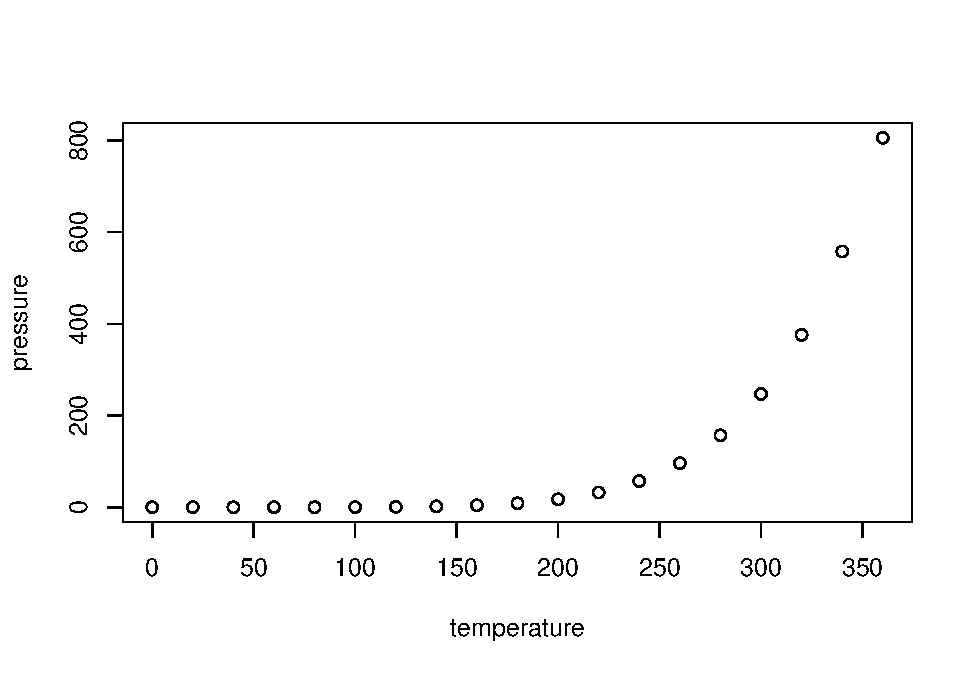
\includegraphics{index_files/figure-latex/pressure-1.pdf}

Note that the \texttt{echo\ =\ FALSE} parameter was added to the code
chunk to prevent printing of the R code that generated the plot.

\end{document}
